\documentclass[tikz,border=10pt]{standalone}
\usepackage{tikz}
\usetikzlibrary{positioning,fit,backgrounds,shadows,calc}

\begin{document}
\begin{tikzpicture}[
    cell/.style={
        draw=gray!30,
        rounded corners=3pt,
        inner sep=5pt,
        fill=white,
        drop shadow={shadow xshift=1pt, shadow yshift=-1pt, opacity=0.2},
    },
    image/.style={
        draw=gray!50,
        fill=gray!20,
        minimum width=8cm,
        minimum height=5cm, % 16:10 aspect ratio
        align=center,
        font=\large
    },
    desc/.style={
        text width=8cm,
        align=center,
        font=\small
    },
    column title/.style={
        font=\bfseries\large,
        align=center
    },
    row title/.style={
        font=\bfseries\large,
        align=center,
        rotate=90
    }
]


\def\colOne{5}
\def\colTwo{14}
\def\colThree{23}
\def\colFour{32}

\def\rowOne{-6}
\def\rowTwo{-13.5}
\def\rowThree{-21}

\def\deviceOne{Intel i9-13900KF with 64 GB RAM and RTX 4090 GPU}
\def\deviceTwo{Intel i9-13980HX with 32 GB RAM and RTX 4060 Laptop GPU}
\def\deviceThree{Apple M1 Max}

% Column titles - moved down closer to the first row and centered over columns
\node[column title] (col1) at (\colOne,-2) {NeRF Blender Lego};
\node[column title] (col2) at (\colTwo,-2) {NeRF Blender Chair};
\node[column title] (col3) at (\colThree,-2) {Mip360 Bicycle};
\node[column title] (col4) at (\colFour,-2) {Mip360 Garden};

% Row titles - kept far left
\node[row title] (row1) at (0,\rowOne) {CUDA};
\node[row title] (row2) at (0,\rowTwo) {DirectX};
\node[row title] (row3) at (0,\rowThree) {Metal};

% Row 1
\begin{scope}[local bounding box=row1cells]
    % Cell (1,1)
    \node[cell] (cell11) at (\colOne,\rowOne) {
        \begin{tikzpicture}
            \node[image] (img11) {
                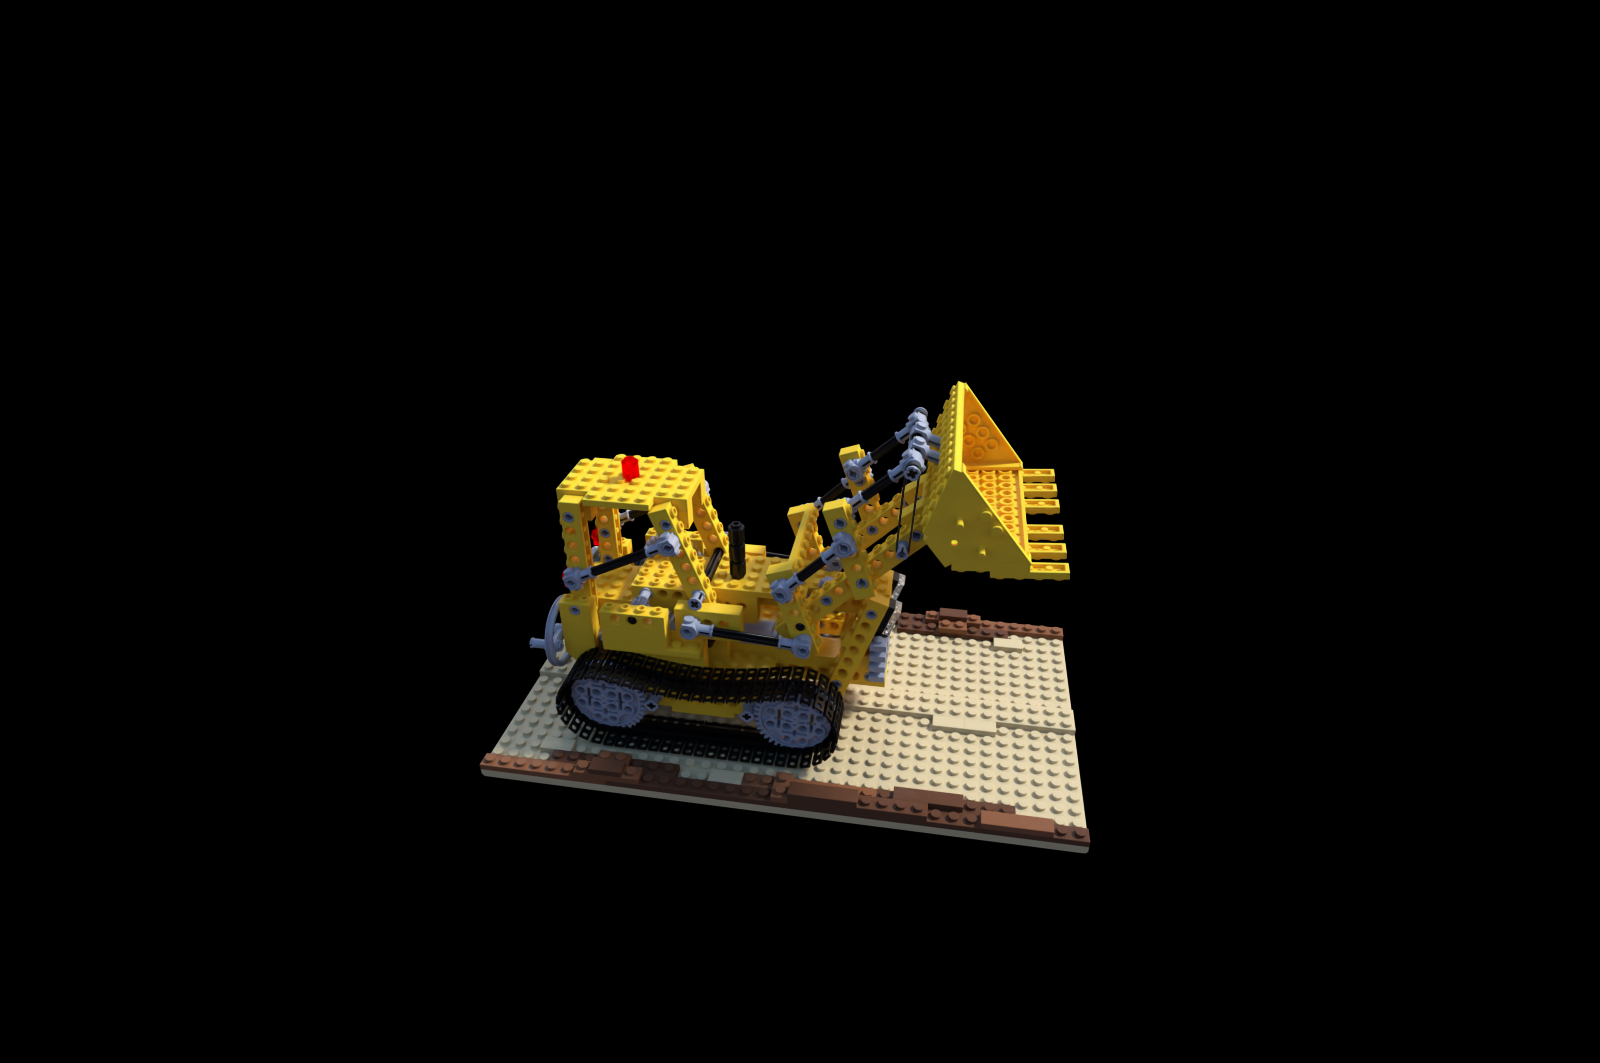
\includegraphics[width=8cm,height=5cm]{nerf_blender_lego_30000_cuda.png}
            };
            \node[desc, below=0.05cm of img11] (desc11a) {Rendered by \deviceOne };
            \node[desc, below=0.01cm of desc11a] (desc11b) {\bf FPS };
        \end{tikzpicture}
    };
    
    % Cell (1,2)
    \node[cell] (cell12) at (\colTwo,\rowOne) {
        \begin{tikzpicture}
            \node[image] (img12) {
                \includegraphics[width=8cm,height=5cm]{nerf_blender_chair_30000_cuda.png}
            };
            \node[desc, below=0.05cm of img12] (desc12a) {Rendered by \deviceOne };
            \node[desc, below=0.01cm of desc12a] (desc12b) {\bf FPS };
        \end{tikzpicture}
    };
    
    % Cell (1,3)
    \node[cell] (cell13) at (\colThree,\rowOne) {
        \begin{tikzpicture}
            \node[image] (img13) {
                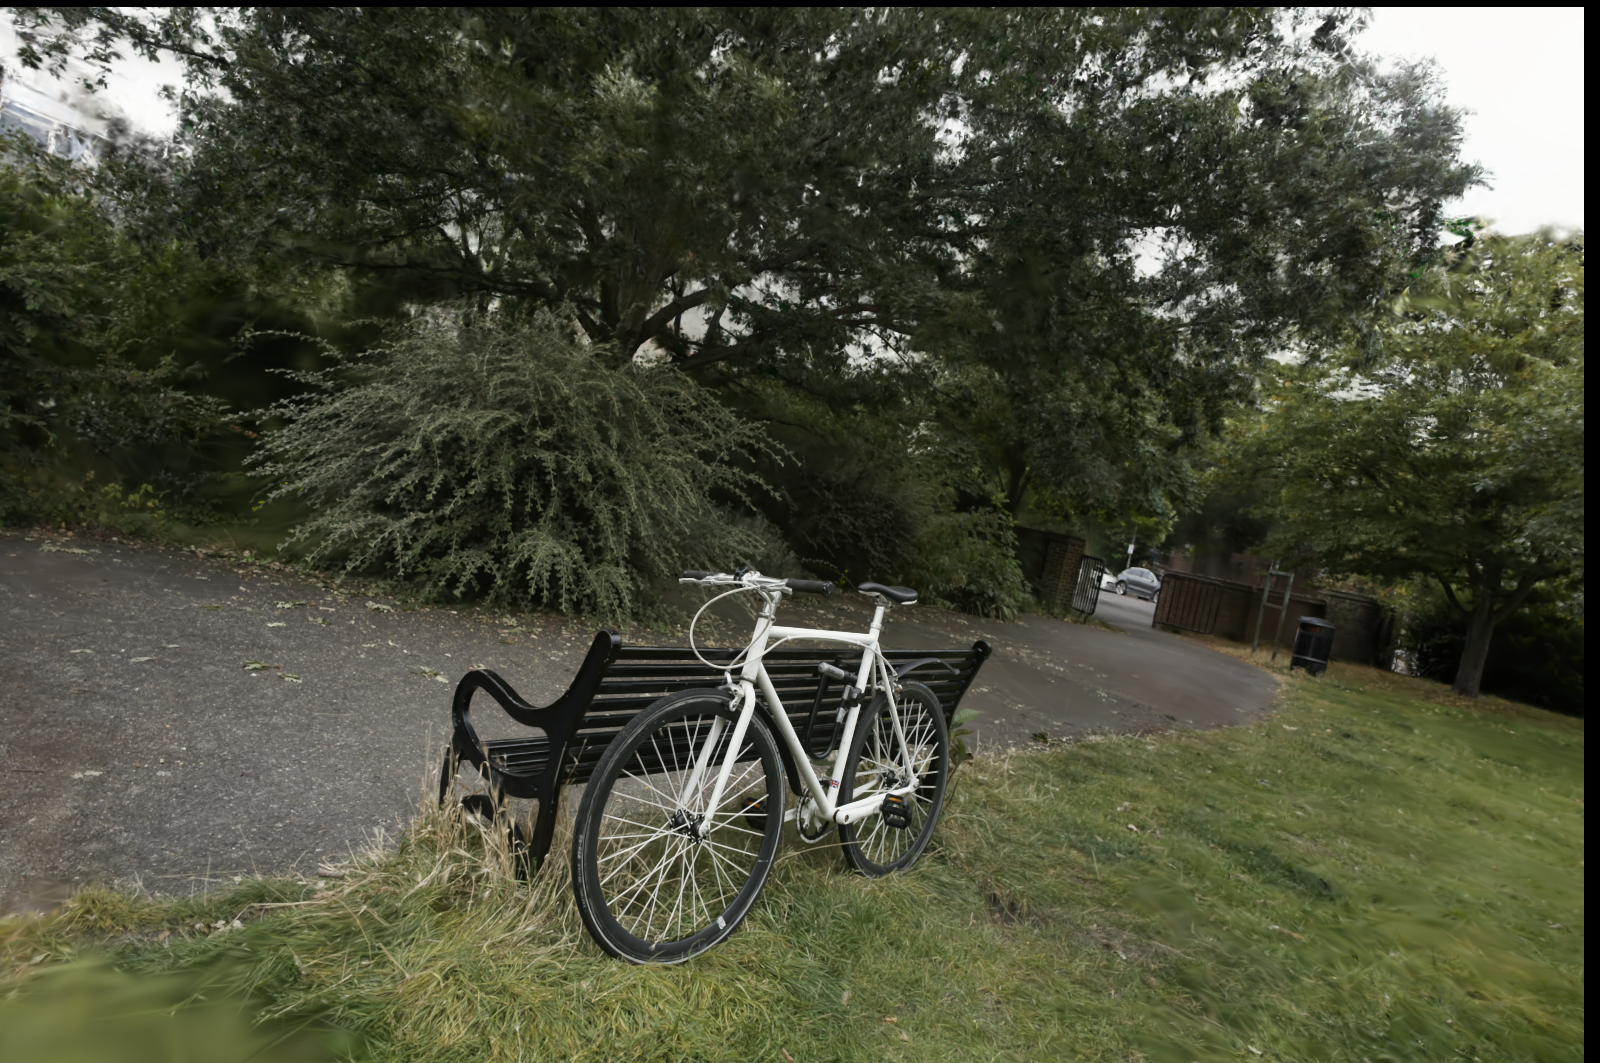
\includegraphics[width=8cm,height=5cm]{mip360_bicycle_30000_cuda.png}
            };
            \node[desc, below=0.05cm of img13] (desc13a) {Rendered \deviceOne };
            \node[desc, below=0.01cm of desc13a] (desc13b) {\bf FPS: 11.70 };
        \end{tikzpicture}
    };
    
    % Cell (1,4)
    \node[cell] (cell14) at (\colFour,\rowOne) {
        \begin{tikzpicture}
            \node[image] (img14) {
                \includegraphics[width=8cm,height=5cm]{mip360_garden_30000_cuda.png}
            };
            \node[desc, below=0.05cm of img14] (desc14a) {Rendered by \deviceOne };
            \node[desc, below=0.01cm of desc14a] (desc14b) {\bf FPS };
        \end{tikzpicture}
    };
\end{scope}

% Row 2
\begin{scope}[local bounding box=row2cells]
    % Cell (2,1)
    \node[cell] (cell21) at (\colOne,\rowTwo) {
        \begin{tikzpicture}
            \node[image] (img21) {
                \includegraphics[width=8cm,height=5cm]{nerf_blender_lego_30000_dx.png}
            };
            \node[desc, below=0.05cm of img21] (desc21a) {Rendered by \deviceOne };
            \node[desc, below=0.01cm of desc21a] (desc21b) {\bf FPS };
        \end{tikzpicture}
    };
    
    % Cell (2,2)
    \node[cell] (cell22) at (\colTwo,\rowTwo) {
        \begin{tikzpicture}
            \node[image] (img22) {
                \includegraphics[width=8cm,height=5cm]{nerf_blender_chair_30000_dx.png}
            };
            \node[desc, below=0.05cm of img22] (desc22a) {Rendered by \deviceOne };
            \node[desc, below=0.01cm of desc22a] (desc22b) {\bf FPS };
        \end{tikzpicture}
    };
    
    % Cell (2,3)
    \node[cell] (cell23) at (\colThree,\rowTwo) {
        \begin{tikzpicture}
            \node[image] (img23) {
                \includegraphics[width=8cm,height=5cm]{mip360_bicycle_30000_dx.png}
            };
            \node[desc, below=0.05cm of img23] (desc23a) {Rendered by \deviceOne };
            \node[desc, below=0.01cm of desc23a] (desc23b) {\bf FPS: 12.54 };
        \end{tikzpicture}
    };
    
    % Cell (2,4)
    \node[cell] (cell24) at (\colFour,\rowTwo) {
        \begin{tikzpicture}
            \node[image] (img24) {
                \includegraphics[width=8cm,height=5cm]{mip360_garden_30000_dx.png}
            };
            \node[desc, below=0.05cm of img24] (desc24a) {Rendered by \deviceOne };
            \node[desc, below=0.01cm of desc24a] (desc24b) {\bf FPS };
        \end{tikzpicture}
    };
\end{scope}


% Row 3
\begin{scope}[local bounding box=row3cells]
    % Cell (3,1)
    \node[cell] (cell31) at (\colOne,\rowThree) {
        \begin{tikzpicture}
            \node[image] (img31) {Image};
            \node[desc, below=0.05cm of img31] (desc31a) {First line of description text};
            \node[desc, below=0.01cm of desc31a] (desc31b) {Second line of description text};
        \end{tikzpicture}
    };
    
    % Cell (3,2)
    \node[cell] (cell32) at (\colTwo,\rowThree) {
        \begin{tikzpicture}
            \node[image] (img32) {Image};
            \node[desc, below=0.05cm of img32] (desc32a) {First line of description text};
            \node[desc, below=0.01cm of desc32a] (desc32b) {Second line of description text};
        \end{tikzpicture}
    };
    
    % Cell (3,3)
    \node[cell] (cell33) at (\colThree,\rowThree) {
        \begin{tikzpicture}
            \node[image] (img33) {
                \includegraphics[width=8cm,height=5cm]{mip360_bicycle_30000_metal.png}
            };
            \node[desc, below=0.05cm of img33] (desc33a) {Rendered by \deviceThree };
            \node[desc, below=0.01cm of desc33a] (desc33b) {\bf FPS: 3.52};
        \end{tikzpicture}
    };
    
    % Cell (3,4)
    \node[cell] (cell34) at (\colFour,\rowThree) {
        \begin{tikzpicture}
            \node[image] (img34) {Image};
            \node[desc, below=0.05cm of img34] (desc34a) {First line of description text};
            \node[desc, below=0.01cm of desc34a] (desc34b) {Second line of description text};
        \end{tikzpicture}
    };
\end{scope}

\end{tikzpicture}
\end{document}